\chapter{Алгоритм построения маршрутов}

\section{Модели данных}
В этом разделе будут описаны 3 способа представления данных о транспортной системе в виде графа, на котором впоследствии будут применятся алгоритмы для построения маршрутов и доступ к которому будет иметь построитель маршрутов.
\subsection{Статичный граф}
В статичном случае каждое ребро взвешенно функцией $c:E \rightarrow R$, и не имеет параллельных ребер. Для каждого ребра $e=(u, v)$ будем писать иногда $c(u, v)$ вместо $c(e)$. Будем называть такой граф простым взвешенным. Вес ребра можно интерпретировать как среднее время движения, требуемое на преодоление сегмента дороги, или как физическую длину. Длина пути $P$ в таком случае равна $c(P)=\sum_{i=1}^{k}c(e_i)$. Путь $P^*$ будет является кратчайшим в том случае, если не существует другого пути $P'$ с такой же стартовой и конечной вершинами, что и у пути $P^*$, такого, что $c(P')<c(P^*)$.

Можно построить граф транспортных рейсов, который будет соответствовать данному случаю. Для этого возьмем за вершину графа транспортный узел, а движение транспорта от одного транспортного узла до другого -- за ребро. За вес ребра будет принята длина сегмента пути, так как она не меняется с течением времени. Далее на таком графе можно применить алгоритм Йена и найти $k$ путей.

К сожалению, такой подход имеет ряд существенных минусов. Во-первых, будет доступна только одна естественная сортировка -- по количеству пересадок, так как в данном случае это будет просто количество ребер. Во-вторых, поддержка временных интервалов потребует дополнительных вызовов алгоритма для того, чтобы гарантированно получить те маршруты, которых попадают в определенные временные границы. В-третьих, это размер графа, который зависит от количества остановок каждого транспорта за период даты продаж.

\begin{figure}[!h]
	\centering
	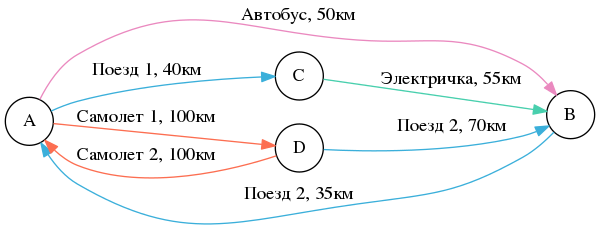
\includegraphics[width=\textwidth]{static_graph_example.png}
	\caption{Статичный граф с 4 узлами и 6 рейсами}\label{fig3}
\end{figure}
\FloatBarrier

\subsection{Граф расписаний}
Традиционно расписания представляются множеством поездов (автобусов, самолетов и т.д.). Каждый поезд посещает последовательность станций (автобусных остановок, аэропортов и т.д.). Для каждой станции, за исключением последней, расписание включает в себя время отбытия и для каждой станции, за исключением первой, включает в себя время прибытия.

Для того, чтобы была возможность математически определить связи, состоящие из нескольких поездов, мы разделим их в элементарные связи. Более формально, мы имеет множество станций $B$, множество остановок $Z_S$ на каждой станции $s \in B$ и множество элементарных связей $C$, чьи элементы $c$ являются кортежами вида $c=\{z_d,z_a,s_d,s_a,\tau_d,\tau_d\}$. Такой кортеж интерпретируется как поезд, который отправляется со станции $s_d$ со временем отбытия $\tau_d$ после остановки $z_d$ и затем следующую остановку $z_a$ на станции $s_a$ с временем прибытия $\tau_a$. Если $x$ обозначает поле кортежа, то $x(c)$ является значением $x$ в элементарном связи $c$. Событие остановки похоже на идентификатор поезда, но на самом деле является более сложным. Определим событие остановки как последовательное прибытие и отбытие поезда со станции, не осуществляя пересадку. Для соответствующего прибытия элементарной связи $c_1$ и отбывающей связи $c_2$ выполняется $z_a(c_1)=z_d(c_2)$. Более того, событие остановки является локальным по отношению к каждой станции. Введем дополнительные события остановки для начала транспортного рейса и для его конца.

\begin{definition}
	Длительность элементарной связи $c$ определяется как $d(c)=\tau_a(c)-\tau_d(c)$.
\end{definition}

На станции или любом другом транспортном узле $s \in B$ возможно совершить пересадку с одного поезда на другой, если время между прибытием и отбытием на станции $s$ больше и равно минимальному времени ожидания пересадки -- $minTransferTime(s)$. Аналогично вводится максимальное время -- $maxTransferTime(s)$. Для простоты дальнейших рассуждений примем $minTransferTime = const_1$ и $maxTransferTime = const_2$.

Пусть $P=(c_1, ..., c_k)$ будет последовательностью элементарных связей. Определим $dep_i(P)=\tau_d(c_i)$, $arr_i(P)=\tau_a(c_i)$, $s_d(P)=s_d(c_1)$, $s_a(P)=s_a(c_k)$, $z_d(P)=z_d(c_1)$, $z_a(P)=z_a(c_k)$, $dep(P)=dep_1(P)$, $arr(P)=arr_k(P)$ и $d(P)=arr(P)-dep(P)$. Таким образом, последовательность $P$ будет называться согласованной связью между станциями $s_d(P)$ и $s_a(P)$, для которой выполняются следующие условия:
\begin{enumerate}
	\item Станция отправления $c_{i+1}$ является станцией прибытия $c_i$.
	\item Для минимального времени пересадки соблюдается либо $z_d(c_{i+1})=z_a(c_i)$, либо $dep_{i+1}(P)-arr_i(P) \geqslant minTransferTime(s_a(c_i))$ 
\end{enumerate}

Для того, чтобы построить из расписания граф, потребуется получить все маршруты поездов. Граф будет иметь 3 вида вершин, каждая из которых будет содержать время и принадлежать станции. Для каждого элементарной связи $c_1=(z_1, z_2, S_1, S_2, \tau_1, \tau_2)$ из станции $s_1$ в станцию $s_2$ на одинаковом поезде мы добавим вершину отправления $S_1d@\tau_1$ на станции $S_1$ со временем отправления $\tau_1$, вершину прибытия $S_2a@\tau_2$ на станции $S_2$ со временем прибытия $\tau_2$ и ребро $S_1d@\tau_1 \rightarrow S_2a@\tau_2$, обозначающее поезду на транспортном средстве со станции $S_1$ на $S_2$. Если транспортное средство продолжает движение со станции $S_2$ во время $\tau_3$, то добавим ребро $S_2a@\tau_2 \rightarrow S_2d@\tau_3$, представляющее собой ожидание транспорта на станции $S_2$. Это возможно независимо от того, насколько мала разница $\tau_3-\tau_2$.

Для каждой вершины отправления $S_2d@\tau$ добавим вершину пересадки $S_2t@\tau$ с тем же временем и добавим ребро $S_2t@\tau \rightarrow S_2d@\tau$ между ними. Также мы добавим ребро $S_2t@\tau \rightarrow S_2t@\tau'$, идущее ко следующей вершине пересадки по возрастаю времени. Такие ребра будем назвать ребрами ожидания (или ребрами пересадки). Теперь для того, чтобы позволить совершить пересадку после прибытия в вершину $S_2a@\tau_2$, добавим ребро к первой вершине пересадки, для которой выполняется $\tau \geqslant \tau_2 + minTransferTime(S_2)$ и $\tau \leqslant \tau_2 + maxTransferTime(S_2)$. Это даст возможность совершить пересадку на любой транспортный рейс.
 
\begin{figure}[!h]
	\centering
	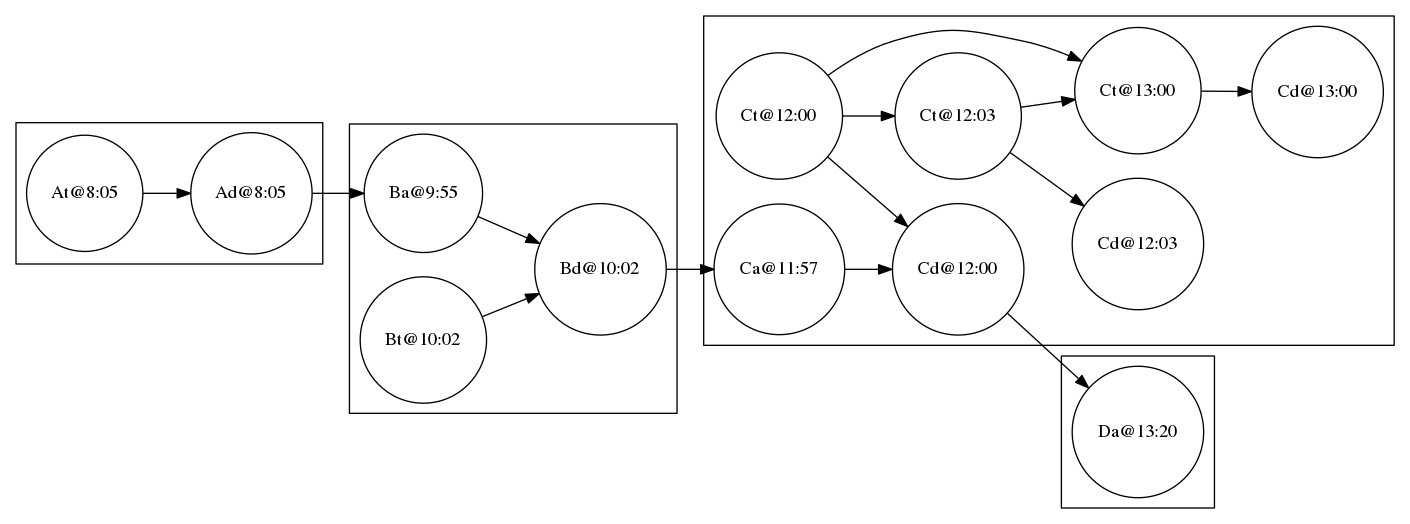
\includegraphics[width=\textwidth]{timetable_graph.png}
	\caption{Для каждого события остановки есть соответствующая вершина. Вес ребра неявно задан по определению длительности элементарной связи. В данном примере $minTransferTime(C)$ равен 10 минутам.}\label{fig4}
\end{figure}
\FloatBarrier 
 
\subsection{Граф рейсов}
Попробуем упростить и в то же время улучшить модель на основе графа расписаний. Заметим, что вершины пересадки $St$ можно удалить из графа без потери информации. Для этого заменим все ребра вида $St@\tau \rightarrow St@\tau'$ на ребра $Sd@\tau \rightarrow Sd@\tau'$. Это возможно сделать, потому что для каждой вершины пересадки $St@\tau$ существует парная ей вершина отправления $Sd@\tau$ с одинаковым временем $\tau$. Также поменяем конец ребер вида $Sa@\tau \rightarrow St@\tau'$ на вершину отправления. Таким образом, поддерживать упорядоченный порядок по времени отправления нужно в самих вершинах отправления.

Следующим шагом улучшения модели будет проведение операции под названием транзитивное замыкание.

\begin{definition}
	В теории графов транзитивным замыканием графа будет является добавление дополнительных ребер между всеми вершинами, между которыми существует путь.
\end{definition}

Наивный способ транзитивного замыкания предполагает добавление ребер между всеми парами вершин отправления $S_id@\tau_i$ и прибытия $S_ja@\tau_j$. Такие ребра будут называться кратчайшими. В них можно хранить информацию о $K_{max}$ кратчайших маршрутах между парой транспортных узлов $S_i$ и $S_j$, где $K_{max}$ -- максимальное количество маршрутов, которые могут быть запрошены клиентским приложением у построителя маршрутов. 

Для того, чтобы сделать полное замыкание графа, нужно построить кратчайшие маршруты от каждой вершины отправления до каждой вершины прибытия. Для такой задачи существует алгоритм Флойда-Уоршелла, который требует $O(n^3)$ времени, где $n$ -- количество вершин\footnote{Улучшенная версия алгоритма требует $O(n^2\log n)$ времени.} и $O(n^3K_{max})$ памяти.

В итоге, несмотря на всю простоту модели, к сожалению, такой подход крайне неэффективно расходует память и требует огромное время на фазу предварительного расчета. 

\begin{figure}[!h]
	\centering
	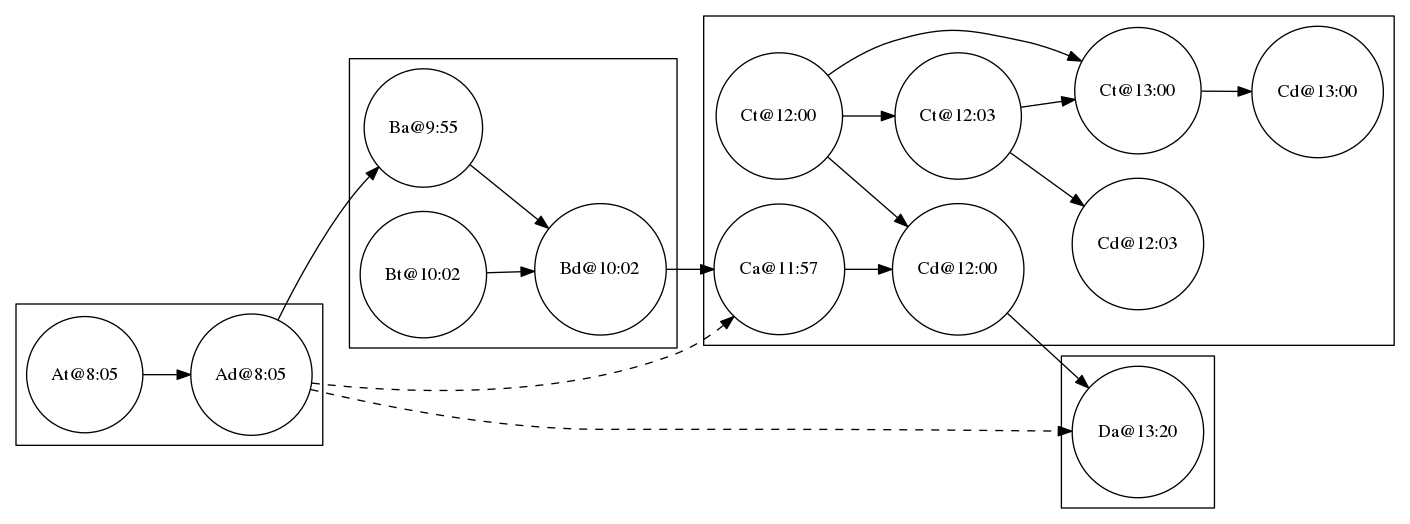
\includegraphics[width=\textwidth]{full_closure_example.png}
	\caption{Для каждого события остановки есть соответствующая вершина. Вес ребра неявно задан по определению длительности элементарной связи. В данном примере $minTransferTime(C)$ равен 10 минутам.}\label{fig4}
\end{figure}

Улучшенный способ транзитивного замыкания работает локально. Вместо того, чтобы добавлять ребра между всеми парами вершин отправления $S_id@\tau_i$ и прибытия $S_ja@\tau_j$ во всем графе, будем добавлять их только между такими вершинами, которые построены на основе конкретного транспортного рейса.

Оценим время и память требуемое для построения такой модели. Пусть $q$ -- количество остановок в одном транспортном рейсе, $n$ -- количество транспортных рейсов. Рассмотрим остановку $z_i$, где i -- номер остановки в транспортном рейсе. В худшем случае от каждой вершины отправления $S_id@\tau$ будет идти $q-i$ ребер до всех оставшихся вершин прибытия $\forall j > i : S_ja@\tau_j$. Аналогично до каждой вершины $S_ia@\tau$ будет идти $i$ ребер от всех вершин прибытия $\forall j < i : S_ja@\tau_j$. Не сложно заметить, что на один транспортный рейс таким образом будет приходиться $\dfrac{q^2}{2}$ ребер. Требуемое время, которое потребуется для построения модели, равно $O(q^2n)$, не считая времени на получение минимальной вершины, а суммарная память -- $O(q^2n)$ для ребер и $O(qn)$ для вершин.

\begin{algorithm}[!h]
	\caption{Алгоритм построения транзитивного замыкания}\label{lst3}
	\begin{algorithmic}
		\Function{Closure}{$runs$, $stops$}
		\For{$ run \in runs$}
		\For{$i = 0$ to $size(stops[run])$}
		\State $S \gets stops[run][i]$ \Comment{получаем из события остановки станцию}
		\State Создаем вершину $S_ia@\tau_i$
		\For{$j = 0$ to $i - 1$}
		\State создаем ребро $S_jd@\tau_j \rightarrow S_ia@\tau_i$
		\EndFor
		\State Создаем вершину $S_id@\tau_i$
		\For{$j = i + 1$ to $size(stops(run))$}
		\State создаем ребро $S_id@\tau_i \rightarrow S_ja@\tau_j$
		\EndFor
		\State $minNode \gets getMinNode(S_id@\tau_i)$ \Comment{получаем минимальную вершину отправления в порядке сортировки по времени}
		\State Создаем ребро пересадки $S_ia@\tau_i \rightarrow minNode$
		\EndFor
		\EndFor
		\EndFunction
	\end{algorithmic}
\end{algorithm}

Попробуем изменить подход и использовать единую вершину остановки. Для этого назовем элементарной остановкой кортеж из 4 элементов $St=(i, r, s, \tau)$, хранящий информацию о номере остановки $i$, транспортном рейсе $r$, станции $s$, а также метки времени $\tau$, которая будет хранить либо время отправления, либо прибытия в зависимости от того, как мы будем её интерпретировать. Задачу о хранении возможных пересадок перенесем из модели графа в модели транспортных рейсов, для которых известны также сами события остановок. Создадим по массив в транспортном рейсе размером с количество его остановок, который будет хранить неупорядоченные списки элементарных остановок.

\begin{algorithm}[!h]
	\caption{Алгоритм построения пересадок}\label{lst4}
	\begin{algorithmic}
		\Function{buildTransfers}{$runs$}
		\For{$ r \in runs$}
		\State $transfers[r] := \emptyset$ \Comment{Список пересадок для транспортного рейса $r$}
		\For{$i = 0$ to $|W(r)| - 1$}
			\State $w := W(r)[i]$
			\State $s := S(w)$ \Comment{по точке маршрута можно получить станцию}
			\If{$i \neq 0$} \Comment{игнорируем $i = 0$, так как только сели на поезд и пересадку делать не нужно в любом случае}
				\State $st_a := (i, R, s, \tau_a(w))$ {Текущая элементарная остановка со временем прибытия}
				\State $T_a(s).put(\tau_a(w), st_a)$ {Помещаем остановку в расписание прибытий станции $s$}
				\For {$(\tau, st') \in T_a(s) : \tau - \tau_a(w) \in [T_{min}(s), T_{max}(s)]$}
					\If{$ R(st') \neq r$} \Comment{Исключаем пересадку на текущий транспорт}
						\State $transfers[i].add(st')$
					\EndIf
				\EndFor
			\EndIf
			\If{$i \neq |W(r)| - 1$} \Comment{не делаем пересадки на поезд, который уже находится на своей конечной станции}
				\State $st_d := (i, R, s, \tau_d(w))$
				\State $T_d(s).put(\tau_a(w), st_d)$
				\For {$(\tau, st') \in T_a(s) : \tau - \tau_d(w) \in [-T_{max}(s), -T_{min}(s)]$}
					\If{$ R(st') \neq r$ \textbf{and} $ i \neq 0$} \Comment{игнорируем $i = 0$, так как только сели на поезд и пересадку делать не нужно в любом случае}
						\State $transfers[i].add(st_d)$
					\EndIf
				\EndFor
			\EndIf
		\EndFor
		\EndFor
		\EndFunction
	\end{algorithmic}
\end{algorithm}

Также нам потребуется хранить 2 структуры данных с поддержкой быстрого поиска элементов в определенной границе. Такой структурой данных может быть красно-черное дерево, поддерживающее поиск элемента за $O(\log n)$, или аналогичный по асимптотике и возможностям список с пропусками. Обе эти структуры помогут быстро находить элементарные остановки во множестве событий прибытия $T_a(s)$ и отбытия $T_d(s)$ на станцию $s$.

Рассмотрим, как теперь будет строиться модель. Построение модели можно реализовать инкрементально, то есть добавлять в модель по одному транспортному рейсу. Для каждого такого рейса создается массив $transfers$, который хранит на $i$ позиции список элементарных остановок отправления, на которые можно пересесть с текущего рейса на $i$ точке маршрута. Пустой список означает, что либо в точке маршрута другой транспорт не останавливается, либо он не подходит по критериям пересадки, то есть не соблюдаются допустимые интервалы времени, связанные с $T_{min}$ и $T_{max}$. Для каждого рейса выполняется обход его маршрутных точек с обновляем пересадок в каждой из них.
\FloatBarrier 

\section{Построение маршрутов}
Теперь у нас есть эффективная модель в виде графа рейсов для хранения информации о транспортной сети. На каждой станции поддерживается несколько структур данных для определения прибывающих и отбывающих поездов по конкретному интервалу времени. Также для каждого транспортного рейса можно быстро узнать возможные пересадки на пути всего следования поезда. Попробуем придумать эффективный алгоритм поиска маршрутов на заданной модели.

\subsection{Дополнение временных интервалов}
Типичный запрос к построителю маршрутов выглядит как кортеж из 5 элементов $q = (s_d, t_d, s_a, t_a, k)$, где $s_d$ и $s_a$ -- станции отправления и прибытия соответственно, $t_d=(\tau_{d1}, \tau_{d2})$ и $t_d=(\tau_{a1}, \tau_{a2})$ -- требуемые интервалы времени, $k$ -- количество маршрутов. Временные интервалы бывают 3 типов:
\begin{enumerate}
	\item Фиксированные
	\item Полубесконечные
	\item Бесконечные
\end{enumerate}

\begin{algorithm}[!h]
	\caption{Приведение интервалов к фиксированному виду}\label{lst5}
	\begin{algorithmic}
		\Function{normalizeTime}{$t_a$, $t_d$}
		\If{$t_{d1} = -\infty$ \textbf{or} $ t_{d1} < T_{now} $}
			\State $t_{d1} := T_{now}$
		\EndIf
		\If{$t_{a2} = \infty$ \textbf{or} $t_{a2} > T_{end}$}
			\State $t_{a2} := T_{end}$
		\EndIf
		\If{$t_{d2} = \infty$ \textbf{or} $t_{d2} > T_{end}$}
			\State $t_{d2} := t_{a2}$
		\EndIf
		\If{$t_{a1} = \infty$ \textbf{or} $t_{a1} < T_{now}$}
			\State $t_{a1} := t_{d1}$
		\EndIf
		\EndFunction
	\end{algorithmic}
\end{algorithm}

Фактически бесконечность в данном случае условная, потому что время построителя маршрутов всегда ограничено снизу текущим временем построителя $T_{now}$, а сверху -- временем конца продаж $T_{end} = T_{now} + T_{len}$, где $T_{len}$~-- интервал продажи билетов. Для упрощения работы с интервалами имеет смысл привести их к фиксированному типу\footnote{Для чего это сделано будет более понятно в следующей главе с конкретной реализацией}.
\FloatBarrier 

\subsection{Фаза инициализации}
Идея алгоритма состоит в следующем: будем генерировать состояния, в которых можем находиться на пути следования до точки назначения. В процессе генерации будем осуществлять фильтрацию маловероятных и невозможных состояний с точки зрения требований к маршруту.

В качестве допустимого состояния будет выступать кортеж из двух элементов $e=(st, m)$, где $st$ -- элементарная остановки, $m$ -- количество совершенных пересадок. 

В процессе работы нам потребуется множество вспомогательных структур данных, в которые будут записываться промежуточные результаты. Часть из них будет являться пересадочными массивами. Под этим термином подразумеваются массивы, индекс в которых будет указывать на текущее число рассматриваемых пересадок. Например, элемент массива $array[3]$ будет хранить данные для состояний, в которых уже совершили 3 пересадки.

\begin{itemize}
	\item $expanded$ -- пересадочный массив множеств посещенных состояний;
	\item $explored$ -- пересадочный массив множеств рассмотренных состояний
	\item $queue$ -- очередь состояний;
	\item $pathsCount$ -- пересадочный массив хеш-таблиц для остановок, хранящий число возможных маршрутов;
	\item $successors$ -- пересадочный массив хеш-таблиц для остановок, хранящий список прямых сегментов;
	\item $predecessors$ -- пересадочный массив хеш-таблиц для остановок, хранящий список обратных сегментов;
\end{itemize}

\subsubsection{Дополнительные модели}
Помимо структур данных нам потребуются несколько новых моделей, в которых мы будем хранить совершаемые действия, чтобы прийти в некоторое состояние $e$. Такие модели будем называть сегментами. В общем случае будет существовать 2 вида сегментов:
\begin{enumerate}
	\item \textbf{Прямой сегмент} ($A-B-C$). Он будет определять действия, совершаемые в процессе обхода графа от событий отправления. Он потребуется нам при сортировке по времени отправления;
	\item \textbf{Обратный сегмент} ($B-C-D$). Он будет определять действия, совершаемые в процессе обхода графа от событий прибытия. Он потребуется нам для всех остальных видов сортировок;
\end{enumerate}

Каждый сегмент состоит из 3 элементарных остановок. Остановка $A$ является событием отправления 1 поезда, $B$ -- его прибытием, $C$ -- это отправление 2 поезда, $D$ -- прибытие. Можно заметить, что часть $B-C$ совпадает у обоих сегментов. Эта часть является неявным событием пересадки, с помощью которого можно однозначно конвертировать сегменты друг в друга, а также находить пересечения. Как будет показано позже, это поможет реализовать двунаправленный обход графа рейсов.

\begin{figure}[!h]
	\centering
	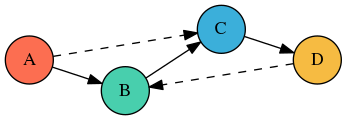
\includegraphics[width=0.5\textwidth]{segments_example.png}
	\caption{Совмещение прямого и обратного сегментов. Пунктирные линии показывают следующее состояние, которое будет добавлено в очередь.}\label{fig4}
\end{figure}

На самом деле любая сортировка может быть выполнена с наличием только одного вида сегментов, потому что путем их обхода можно из одного вида получить другой.

\subsubsection{Заполнение вспомогательные структур}
Перед фазой обхода необходимо произвести инициализацию необходимых данных. Эта операция будет происходить один раз на каждый запрос $q$.

Во-первых, должны быть начальные состояния, чьи остановки $st$ удовлетворяют запросу $q$ и приведены к фиксированному типу. Аналогично, требуется создать конечные состояний (если обход графа будет с конца). Во втором случае возникает проблема из-за того, что зная какие конечные остановки $st'$, мы не знаем, при каком количестве пересадок $m$ они совершаются. В таком случае нам придется создать состояния для всех возможных вариантов, то есть $\forall m : m \in [0, M]$, где $M$ -- максимально допустимое количество пересадок. 

Во-вторых для некоторых эвристических оптимизаций будет полезно сохранить список начальных и конечных транспортных узлов, чтобы не проверять каждый раз непосредственно множества состояний.

\begin{algorithm}[!h]
	\caption{Заполнение вспомогательных структур}\label{lst5}
	\begin{algorithmic}
		\For {$s \in sources$}
			\State $departures.add(P(s))$ \Comment{Добавляем транспортный узел в список узлов отправления}
			\State $pathsCount[0].put(s, 1)$ \Comment{Из остановки можно доехать в саму себя за 0 пересадок только 1 способом}
			\State $st = (s, 0)$ \Comment{Создаем состояние с событием отправления $s$ и $0$ совершенных пересадок}
			\State $explored.add(st)$ \Comment{Добавляем состояние в список рассмотренных}
			\State $queue.add(st)$ \Comment{Добавляем в очередь на обработку}
		\EndFor
		\For {$t \in targets$}
			\State $arrivals.add(P(t))$ \Comment{Добавляем транспортный узел в список узлов прибытия}
		\EndFor
	\end{algorithmic}
\end{algorithm}

\FloatBarrier
\subsection{Фаза обхода}
В фазе обхода мы начинаем рассматривать в произвольном или упорядоченном порядке все доступные на текущий момент состояния. Соответственно состояния берутся из очереди $queue$, которая может быть обычным связным списком или двоичной кучей. Для простоты будет рассматривать первый вариант, где порядок рассмотрения определяется порядком добавления в очередь. Одним из основных критериев остановки является то, что очередь стала пустой. Это говорит нам о том, что мы рассмотрели все возможные состояния, подходящие под требования запроса $q$, или не может сгенерировать новые.

Для примера рассмотрим прямой обход графа рейсов. После извлечения очередного состояния $v=(st, m)$ добавим его во множество посещенных состояний $expanded$. Теперь нужно сделать проверку, что не остановка $st$ из состояния $v$ не совершается в одном из конечных транспортных узлов. В противном случае, можно перейти к рассмотрению следующего состояния. Получим по остановке $st$ все возможные прямые сегменты, где $A = st$. 

Для каждого прямого сегмента рассмотрим остановку отправления второго поезда $C$. Следует заметить, что сегмент либо является пересадочным, либо $I(A) < I(C)$. Это следует из того, что $R(A)=R(C)$ и $T(A) \leqslant T(C)$ для любого сегмента. Если сегмент пересадочный, то новое количество пересадок $m' = m + 1$. Далее следует проверить, что состояние $v'=(C, m')$ отсутствует в списке посещенных состояний. Если это так, то можно добавить в список прямых сегментов $successors[m]$ текущий рассматриваемый сегмент. Аналогично, можно сделать для обратного сегмента и $predessors[m']$\footnote{В целях оптимизации памяти следует заполнять только один вид сегментов для соответствующего прямого или обратного обхода графа рейсов.}. Формально это соответствует следующей динамике:

\[
predessors[m'][C]=\{\langle A, m\rangle\ |\ \exists \langle A, m \rangle \rightarrow \langle C, m' \rangle\}
\]

Аналогично, можно подсчитать количество путей:
\[
pathsCount[m'][C] = pathsCount[m][A] + pathsCount[m'][C];
\]

На последней стадии новое состояние $v'$ можно добавить в очередь $queue$, предварительно проверив, что оно отсутствует в списке рассмотренных состояний. Это предотвратит экспоненциальное рост очереди.

\begin{algorithm}[!h]
	\caption{Фаза обхода графа рейсов}\label{lst5}
	\begin{algorithmic}
		\Function{fillLevel}{$level$, $k$}
		\For{$t \in targets$}
		\State $incomming := predecessors[k][t]$;
		\For {$s \in incoming$}
		\State $level.add(k, s)$
		\EndFor
		\EndFor
		\EndFunction
	\end{algorithmic}
\end{algorithm}

Теперь рассмотрим более подробно получение списка всех возможных прямых сегментов по остановке $A$. В общем виде остановка $A=(i, r, s, \tau)$, поэтому мы можем получить список маршрутных точек $W(r)$ транспортного рейса $r$. Далее начнем рассматривать каждую такую точку с номерами больше $i$, так как префикс маршрута, включающий точки с $0$ до $i$ уже пройдены поездом. Для каждой маршрутной точки $w \in W(r)$ известен транспортный узел $S(w)$, поэтому мы можем проверить, чтобы $S(w)$ не входили в списки станций отправления и прибытия. Для этого у нас имеются множества $departures$ и $arrivals$, так как там не собираемся делать пересадку. Стоит отметить, что могут существовать случаи, когда маршрут делает петлю, посещает одну и ту же станцию несколько раз, но в рамках этой работы будем считать, что они отсутствуют. Иначе бы было необходимо различать такие маршрутные точки. Сделать это можно было бы по временной метке или номеру. В данный момент следует указать, что прямые и обратные сегменты имеют еще 2 вида:
\begin{enumerate}
	\item \textbf{Конечный сегмент}. Он будет определять действие, когда мы уже находимся на транспорте в точке отправлений и не делаем пересадку.
	\item \textbf{Пересадочный сегмент}. Аналогичен предыдущему виду за исключением того, что пересадка на другой транспорт делается.
\end{enumerate}

Тогда в случае, когда одна из маршрутных точек является конечной станцией, то можно создать конечный сегмент. Учитывая, что сегмент хранит 3 остановки, то прямой конечный сегмент будет выглядеть как $A-C-C$.

Теперь можно из графа рейсов получить через $T_a(S(w))$ и $T_d(S(w))$ списки элементарных остановок прибытия и отбытия и сгенерировать все оставшиеся пересадочные сегменты. Для этого можно воспользоваться массивом $transfers$, который присутствует у каждого транспортного средства. Тогда остановка $A$ известна заранее, $B$ получается из текущей маршрутной точки, а $C$ берется из данного массива. В конце все полученные сегменты следует отфильтровать, что будет описано в данной главе позже.

\begin{algorithm}[!h]
	\caption{Получение списка прямых сегментов}\label{lst5}
	\begin{algorithmic}
		\Function{successors}{$departures$, $A$, $arrivals$}
		\For{$t \in targets$}
		\State $incomming := predecessors[k][t]$;
		\For {$s \in incoming$}
		\State $level.add(k, s)$
		\EndFor
		\EndFor
		\EndFunction
	\end{algorithmic}
\end{algorithm}

\section{Сортировка маршрутов}
По постановке задачи маршруты требуется строить инкрементально в порядке сортировки. Виды сортировок были описаны в обзоре данной работы. Все дополнительные структуры данных, полученные на предыдущем этапе, потребуются теперь для реализации фазы построения и сортировки маршрутов. Из-за того, что все предикаты сортировок известны нам заранее, мы можем придумать и реализовать необходимый алгоритм для каждого из них, который будет эффективнее абстрактного аналога. Рассмотрим каждый вид сортировки подробнее.

\subsection{Количество пересадок}
Как было сказано ранее, данный вид сортировки является наиболее простым из представленных, потому что на фазе обхода графа рейсов заполнение списков прямых и обратных сегментов выполнялось в естественном порядке из-за пересадочных массивов. Тогда мы можем инкрементально строить маршруты в таком же порядке.

Для начала на данной фазе нам потребуются дополнительные модели. Будем называть их слоями. В общем случае слои будут содержать концы сегментов (прямых или обратных), по которым можно деструктивно итерироваться, то есть производить обход с удалением не нужных сегментов. Всего 2 вида слоев:
\begin{enumerate}
	\item \textbf{Произвольный слой}. Имеет доступ к сегментам в порядке их добавления.
	\item \textbf{Упорядоченный слой}. Имеет доступ к сегментам, сортированных по их остановкам или прочим параметрам.
\end{enumerate}

Теперь определим функцию, которая производит заполнение слоя с помощью множества обратных сегментов. Основная идея в том, чтобы обойти все конечные элементарные остановки прибытия и их обратные сегменты для каждого количества совершенных пересадок. Таким образом, сегменты $A-B-C$, где состояния $v=(C, m)$ для остановок $C$ имеют меньшее количество пересадок $m$, будут в начале слоя.
\begin{algorithm}[!h]
	\caption{Заполнение переданного слоя}\label{lst5}
	\begin{algorithmic}
		\Function{fillLevel}{$level$, $k$}
		\For{$t \in targets$}
			\State $incomming := predecessors[k][t]$;
			\For {$s \in incoming$}
				\State $level.add(k, s)$
			\EndFor
		\EndFor
		\EndFunction
	\end{algorithmic}
\end{algorithm}

Для того, чтобы начать восстановление (построение) маршрутов нужно создать и заполнить корневой слой. Для сортировки по количеству пересадок будем оперировать произвольными слоями. Мы хотим поддерживать для каждого вида сортировки следующие направления: восходящую (ASC) и нисходящую (DESC). В таком случае, для текущего вида сортировки можно просто совершать заполнение корневого слоя по возрастанию количества пересадок (ASC) или по убыванию (DESC).

\begin{algorithm}[!h]
	\caption{Подготовка сортировки по количеству пересадок}\label{lst5}
	\begin{algorithmic}
		\Function{sortedByTransfersCount}{$level$, $k$}
		\State $unvisited := \emptyset$ \Comment{случайный уровень}
		\If {$direction = ASC$}
			\For {$i = 0$ \textbf{to} $maxTransfersCount$}
				\State \Call{fillLevel}{unvisited, i}
			\EndFor
		\Else
		\For {$i = maxTransfersCount$ \textbf{downto} $0$}
			\State \Call{fillLevel}{unvisited, i}
		\EndFor
		\EndIf
		\State \Return $unvisited$
		\EndFunction
	\end{algorithmic}
\end{algorithm}

Дополнительно нам потребуется новый вид состояния -- построения (СП). Им будет являться кортеж $v_b=(v_b', s, m)$, который хранит ссылку на предыдущее состояние построения $v_b'$, сегмент $s$ и количество совершенных пересадок $m$. Оно будет нужно для того, чтобы можно было сохранять и восстанавливать дерево восстановления маршрутов.

Итак, у нас есть заполненный корневой слой и множество обратных сегментов. Теперь мы можем построить функцию, которая будет возвращать очередной маршрут в порядке сортировки по количеству пересадок. Основная идея в том, чтобы рассматривать слои и строить новые жадным способом, то есть слой будет в кандидатах на рассмотрение до сих пор пока не станет пустым. Дополнительные эвристики, которые позволят ускорить данный шаг будут рассмотрены позже.

\begin{algorithm}[!h]
	\caption{Строим и возвращаем следующий маршрут по множеству обратных сегментов}\label{lst5}
	\begin{algorithmic}
		\Function{backwardNext}{$level$, $k$}
		\While {$stack \neq \emptyset$}
		\State $level := stack.peek()$ \Comment{получаем текущий уровень в стеке}
		\If {$level \neq \emptyset$}
		\State $v_b = level.poll()$ \Comment{извлекаем состояние из уровня}
		
		\State $b := v_b.segment.B()$
		\State $t := v_b.transfers$
		
		\If {$departures\text{ содержит }P(b)$} \Comment{Маршрут найден, так как пришли в точку отправления}
		\State $path = \Call{buildFrom}{state, true}$ \Comment{Строим маршрут}
		\State $candidates.add(path)$ \Comment{Добавляем маршрут в список кандидатов}
		\EndIf
		
		\State $incoming := predecessors[t][b]$;
		\If {$incoming \neq \emptyset$}
		\State $level' := \emptyset$ \Comment{создаем новый случайный уровень}
		\For {$s' \in incoming$}
		\If {$s'\text{ является пересадочным}$}
		\State $t' = t + 1$
		\Else
		\State $t' = t$
		\EndIf
		\State $v_b' := (v_b, s', t')$
		\State $level'.add(st')$
		\EndFor
		\State $stack.push(level')$
		\EndIf
		\Else
		\State $stack.poll()$ \Comment{на текущем уровне не осталось состояний, можно подняться выше}
		\EndIf
		\EndWhile
		\EndFunction
	\end{algorithmic}
\end{algorithm}

Создадим стек, который будет хранить сегменты и определять порядок, в котором мы их обрабатываем. На вершине стека будет храниться текущий обрабатываемый уровень. На очередном шаге получаем и удаляем первое по порядку состояние построения из уровня. Так как СП содержит обратный сегмент, то имеется элементарная остановка $B$, транспортный узел которой следует проверить на принадлежность множеству точек отправления $departures$. При положительном ответе можно восстанавливать маршрут и добавлять его в список кандидатов на выдачу в ответ. При данном виде сортировки для такого списка будет просто действовать принцип FIFO\footnote{Акроним First In, First Out -- «первым пришел -- первым ушел»}. Далее по остановке $B$ можно получить список обратных сегментов. По ним создается новый произвольный слой и множество состояний построения, которые будут в него добавлены. На этом этапе для каждого обратного сегмента $s'$ можно создать состояние $v_b'=(v_b, s', t')$, где $t'$ -- количество пересадок, которое получается из текущего количества и того факта, является ли обратный сегмент пересадочным или нет. Новый слой со всеми СП кладется в стек.

\FloatBarrier
\subsection{Время прибытия}
Получение очередного маршрута осуществляется через вызов построителя маршрутов, который выполняет фазу инициализации, фазу обхода, вызывает подготовку для соответствующей сортировки, а затем выполняет фазу восстановления маршрутов, после которой в списке кандидатов на выдачу будет лежать некоторое количество маршрутов. Случай пустого списка означает, что были восстановлены все возможные маршруты. Не сложно заметить, что нужно дополнительно вести счетчик восстановленных маршрутов или удалять очередной восстановленный из списка.

Рассмотрим восстановление маршрута (функция $\Call{buildFrom}$). Это несложная операция выполняет рекурсивный подъем вверх по дереву состояний построения. Так для каждого состояния $v_b$ известно состояние $v_b'$, в котором имеется сегмент. Результатом выполнения функции будет список сегментов и количество пересадок, которые совершаются по ходу движения по маршруту. Далее с этими данными можно восстановить любую информацию о транспортных рейсах или транспортных узлах.

В рамках данной работы использовались куски сегментов $A-B$ и $C-D$ для определения конечной стоимости маршрута, которая зависит от транспорта и пройденного расстояния. К сожалению, честное определение стоимости маршрута -- очень времязатратная операция, а также стоимость не является аддитивной величиной, то есть цена преодоления отрезков $A-B$ и $B-C$ не равна цене отрезка $A-C$ из-за сложных бизнес-правил, поэтому в рамках данной работы сортировка по стоимости не рассматривается.

\begin{figure}[!h]
	\centering
	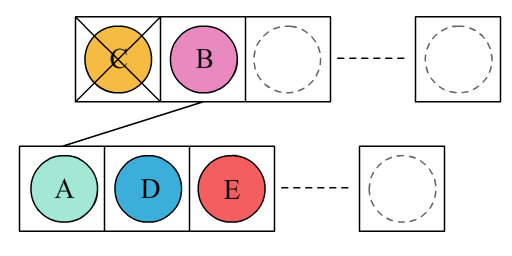
\includegraphics[width=0.5\textwidth]{sorted_by_arrival.png}
	\caption{Стек слоев с состояниями построения.}\label{fig8}
\end{figure}

Текущий вид сортировки похож на предыдущих, но в данном случае мы будем использовать в процессе подготовки упорядоченный корневой слой. В случае прямого обхода графа в качестве предиката сортировки состояний построения можно использовать сравнение элементарных остановок $C=(i, r, s, \tau)$, у которых будут сравниваться их времена отправления $\tau$. Благодаря этому, мы можем без изменений использовать функцию возврата очередного маршрута из предыдущего раздела.

\subsection{Время отправления}
Сортировка по времени отправления во многом похожа на предыдущую. Мы также будем использовать упорядоченный корневой слой, но уже с другим предикатом сравнения -- времени прибытия остановки $A$ (для случая прямых сегментов). Аналогично придется изменить функцию возврата очередного маршрута для случая, когда мы восстанавливаем маршрут по множеству прямых сегментов. Описание похода во многом похоже на рассматриваемый разделе про сортировку по количеству пересадок -- сегменты и их элементарные остановки симметрично заменяются.

\begin{algorithm}[!h]
	\caption{Строим и возвращаем следующий маршрут по множеству прямых сегментов}\label{lst5}
	\begin{algorithmic}
		\Function{forwardNext}{$level$}
		\While {$stack \neq \emptyset$}
			\State $level := stack.peek()$ \Comment{получаем текущий уровень в стеке}
			\If {$level \neq \emptyset$}
				\State $v_b = level.poll()$ \Comment{извлекаем состояние из уровня}
				
				\State $b := v_b.segment.B()$
				\State $t := v_b.transfers$
				
				\If {$arrivals\text{ содержит }P(b)$} \Comment{Маршрут найден, так как пришли в точку отправления}
				\State $path = \Call{buildFrom}{state, true}$ \Comment{Строим маршрут}
				\State $candidates.add(path)$ \Comment{Добавляем маршрут в список кандидатов}
				\EndIf
				
				\State $outgoing := successors[t][b]$;
				\If {$outgoing \neq \emptyset$}
				\State $level' := \emptyset$ \Comment{создаем новый случайный уровень}
				\For {$s' \in outgoing$}
				\If {$s'\text{ является пересадочным}$}
				\State $t' = t + 1$
				\Else
				\State $t' = t$
				\EndIf
				\State $v_b' := (v_b, s', t')$
				\State $level'.add(v_b')$
				\EndFor
				\State $stack.push(level')$
				\EndIf
			\Else
				\State $stack.poll()$ \Comment{на текущем уровне не осталось состояний, можно подняться выше}
			\EndIf
		\EndWhile
		\EndFunction
	\end{algorithmic}
\end{algorithm}

Эвристическая оптимизация.TODO

\FloatBarrier
\subsection{Время в пути}
Во всех предыдущих видах сортировок мы обходились созданием корневого слоя, который позволял задать порядок построения маршрутов. Это было возможно, потому что на фазе обхода мы получали естественную сортировку по количеству пересадок, а для остальных видов нужно была лишь информация о началах или концах маршрутов. В сортировка по времени в пути требуется информация о маршруте целиком, так как длительность маршрута состоит из длительностей прохождения отдельных его сегментов. К счастью, в отличие от стоимости длительность -- аддитивная величина, то есть время прохождения отрезков $A-B$ и $B-C$ равно времени, которое тратится на $A-C$. Это дает нам возможность запоминать время прохождения смежных сегментов.

Для данного вида сортировки потребуется добавить новую модель -- ленивое состояние построения (ЛСП). Оно будет во многом похоже на обычное состояние построения, используемое в других сортировках. Основное отличие в том, что каждое состояние будет дополнительно хранить список префиксов уже построенных маршрутов в количестве $K_{max}$ штук, где $K_{max}$ -- максимальное количество запросов, которое может быть в поисковом запросе $q$. В общем случае такое состояние будет хранить приоритетную очередь ленивых ссылок $v_q$ и список уже готовых обычных состояний построения $v_c$. Ленивая ссылка -- это ещё одна новая модель данных. Она будет хранить сегмент, исходящих из ЛСП, по которому можно в него прийти, если начинать построение с конца графа рейсов. Также она должна хранить последнее построенное СП.

\begin{figure}[!h]
	\centering
	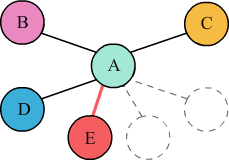
\includegraphics[width=0.4\textwidth]{sorted_by_time.png}
	\caption{ЛСП $A$ с очередью из 4 ленивых ссылок и 2 посчитанными СП. На само ЛСП $A$ тоже ведут 2 ленивые ссылки.}\label{fig8}
\end{figure}

Для подготовки к восстановлению маршрутов нужно рекурсивно обойти конечные элементарные остановки по обратным сегментам и построить для каждой по ЛСП. Для каждого обратного сегмента будет создана ленивая ссылка, содержащая этот сегмент и соединяющая смежные остановки. После нужно принудительно вызвать для всех конечных остановок получение очередного префикса. Если в каждой ленивой ссылке хранить текущий номер построенного префикса маршрута, тогда при условии, что текущий номер меньше количества префиксов в списке $v_c$, можно просто вернуть элемент из списка, иначе рекурсивно вызвать процедуру для минимального (ASC) или максимального (DESC) элемента из очереди $v_q$. Так как для каждой ЛСП доступен только префикс маршрута и время в пути аддитивно, то в качестве предиката сравнения для очереди $v_q$ будет использоваться сравнение длительности префиксов маршрутов в соответствии с требуемым направлением сортировки.

Для удобства следует создать фиктивное ленивое состояние построение, которое назовем корневым. От корневого состояния будут вести ленивые ссылки с нулевыми сегментами\footnote{В общем виде они должны быть нейтральными элементами по отношению к сложению.}. Тогда получение очередного маршрута будет являться вызовом функции для построения префикса от корневого состояния. Если очередь для этого состояния стала пустой, то все маршруты построены.

\section{Построение фильтров}
Построение фильтров также, как и поиск маршрутов, состоит из двух фаз: предварительного расчета и основной. В первом случае модели данных, которые отвечают за транспортные средства переводятся в удобные и компактные модели, которые будут использоваться при непосредственном поиске маршрутов. Во втором случае готовые структуры данных будут позволять на этапе фазы обхода графа рейсов собирать композитные фильтры для каждой остановки с помощью динамического программирования. Также как и случае подсчета количества маршрутов мы построим динамику, которая будет позволять определять доступные параметры фильтрации для пары элементарных остановок.

\subsection{Косвенные признаки}
В фазе предварительного расчета мы будем извлекать косвенные признаки из моделей транспортных средств. Как было описано в главе 1, такими признаками может быть тип транспорта, номер поезда или тип места в самолете и т.д. Для удобной работы с ними мы разделим все признаки по функциональным типам, то есть, например, признак "перевозчик" у поезда и самолета будут отнесены к разных типам признаков. Это позволит нам логически отделять на этапе отдачи результата клиентскому приложению.

В качестве компактной модели свойств $Pr=\{(t,\{(v, c)\})\}$, хранящей признаки, будет выбрана хеш-таблица из типа признака $t$ в хеш-таблицу значений признака $v$ в количество свободных мест $c$, которые удовлетворяют ему. Например, есть 1 поезд с 3 вагонами (один вагон имеет 20 мест): 2 из них купе, 1 - плацкарт. Из них в плацкарте половина верхних мест, а другая половина - нижних. Тогда будет создан объект свойств для поезда со следующими записями:
\begin{itemize}
	\item Тип транспорта
	\begin{itemize}
		\item (Поезд, 60)
	\end{itemize}
	\item Тип вагона
	\begin{itemize}
		\item (Купе, 40)
		\item (Плацкарт, 20)
	\end{itemize}
	\item Тип места
	\begin{itemize}
		\item (Верхнее, 20)
		\item (Нижнее, 20)
	\end{itemize}
\end{itemize}

Как можно заметить на данном примере, свойства не хранятся в виде иерархии функциональных зависимостей. Это сделано для экономного расхода памяти, а также для упрощения операций со свойствами в процессе выполнения динамики по свойствами. Функциональные зависимости известны заранее и задаются вручную в специальном объекте, о котором речь пойдет позже.

Теперь нужно ввести 2 операции в пространстве свойств признаков, которые будут называться минимум и максимум. Обе операции будут являться ассоциативными, то есть:
\[
(x\circ y)\circ z=x\circ(y\circ z)\text{ для любых элементов }x,\;y,\;z.
\]

Минимум на свойствах работает как минимум количества свободных мест по всем парам признаков $\langle t, v \rangle$. При этом работает правило дополнения, то есть если пара присутствует в свойстве $A$, но отсутствует в $B$, то берется число свободных мест из $A$.

\begin{algorithm}[!h]
	\caption{Минимум из пары свойств}\label{lst5}
	\begin{algorithmic}
		\Function{min}{$Pr_a$, $Pr_b$}
		\If{$Pr_a = \emptyset$}
			\State \Return $Pr_b$
		\EndIf
		\If{$Pr_b = \emptyset$}
		\State \Return $Pr_a$
		\EndIf
		\State $Pr_r := \emptyset$ \Comment{Результирующее свойство}
		\For{$ \langle t, v\rangle : Pr_a \cap Pr_b$}
			\State $Pr_r[t][v] = min(Pr_a[t][v], Pr_b[t][v])$
		\EndFor
		\For{$ \langle t, v\rangle : Pr_a \setminus Pr_b$}
			\State $Pr_r[t][v] = Pr_a[t][v]$
		\EndFor
		\For{$ \langle t, v\rangle : Pr_b \setminus Pr_a$}
			\State $Pr_r[t][v] = Pr_b[t][v]$
		\EndFor
		\State \Return $Pr_r$
		\EndFunction
	\end{algorithmic}
\end{algorithm}

Максимум на свойствах работает аналогично минимуму, только для количества свободных мест операция меняется на максимум.

\subsection{Осуществление фильтрации}
В фазе обхода при построении маршрутов для каждой элементарной остановки генерировались все возможные сегменты, которые являлись пересадочными и конечными. Таким образом, чтобы избежать попадание в следующую элементарную остановку, нужно фильтровать соответствующий сегмент, поэтому в процессе генерации каждому сегменту должно сопоставляться свойство, хранящее признаки для транспортного средства, отправляющегося из остановки $A$\footnote{Для упрощения рассматривается прямой сегмент, для обратного будет остановка прибытия $D$.}

В итоге, мы должны хранить свойства для каждого отрезка пути, соединяющего смежные маршрутные точки. Так как сегмент является множеством последовательно соединенных отрезков пути следования, то свойство сегмента является минимумом из всех свойств отрезков, входящих в него:
\[
Pr_s=\min_{i \in s}{Pr_i}
\]

Для того, чтобы ускорить построение свойства сегмента можно воспользоваться деревом отрезков, позволяющее находить результат операции на интервале за $O(\log q)$ времени и требующее $O(2q)$ памяти, где $q$ -- число маршрутных точек транспортного рейса. В качестве операции будет взята операция минимума свойств. Это возможно, так как определенный ранее минимум ассоциативен, так же имеет нейтральный элемент -- пустое свойство (пустую хеш-таблицу). Таким образом, множество свойств является моноидом, который можно применять в дереве интервалов.

\subsection{Функциональные зависимости}
В модели свойств ради ускорения бинарных операций и уменьшения требуемой для хранения памяти используется сжатая форма, из-за которой теряется функциональная связь между отдельными признаками транспортных рейсов. Так каждый поезд состоит из вагонов, каждый вагон из отдельных секций (в случае с купе), а также отдельных мест, которые могут находиться в различных состояниях (свободно, куплено, зарезервировано) и имеют дополнительные признаки (верхнее, нижнее, с розеткой и т.д.). При построении свойств доступных маршрутов требуется, чтобы модель зависимостей также отражалась в конечном результате. Например, мы должны суммировать свободные места с одинаковыми свойствами по всем вагонам, но должны брать максимум по всем поездам. К счастью, такие зависимости известны заранее, поэтому их можно сохранить и использовать только для восстановления структуры.

\begin{figure}[!h]
	\centering
	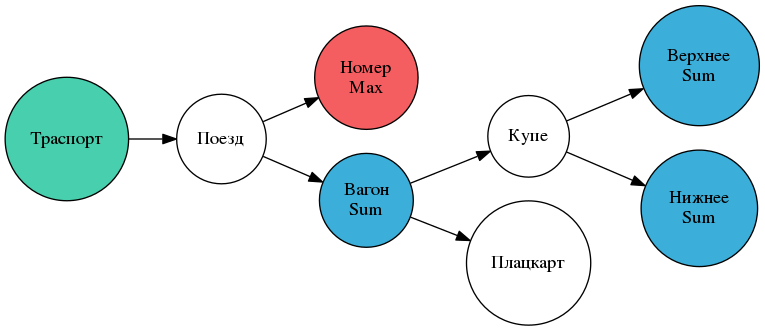
\includegraphics[width=0.9\textwidth]{dependencies.png}
	\caption{Корневой признак ''Транспорт'', функции задаются только для значений признаков.}\label{fig8}
\end{figure}

\chapterconclusion